\chapter{The Standard Model of Particle Physics}\label{chapt:SM}

This chapter provides an introduction to Elementary Particle Physics as described by the Standard Model (SM).
First the particles of the SM are described, then the way they interact is shown. A short introduction
to the physics of the top quark is given in the end.

\section{Introduction. Elementary Particle physics}

The main question which elementary particle physics addresses is '\textit{What is the matter made of?}'
This question was stated many thousands years ago and is still of current interest. First guesses about
the structure of matter were made already in ancient Greece by the philosopher-atomist Demokrit, who
claimed that everything around us consists of tiny undevidable chunks called \textit{atomos}\cite{yangcn}.
But the elementary particle physics (elementary here means unstructured) in a modern sense started with 
J.J. Thomson's discovery of the \textit{electron}\cite{jjthome} in 1897. The electrons were correctly surmised to be constituents
of atoms. A much more detailed picture of the atom structure was obtained after Ernest Rutherford's scattering experiment\cite{rutherford},
proving atom cores to be much smaller than the full atoms and showing that an atom consists of a heavy positively charged core, called 
\textit{nucleus} and very light negatively charged electrons, moving around like satellites. 
The nucleus was later proven to be non-elementary, consisting of elementary particles called \textit{quarks}. 
However, up to date no structure of electron was discovered 
and it is nowadays known as one of the elementary particles. 

Many other elementary particles were subsequently discovered during the last sixty years. Now having an idea 
what the structureless bricks making up matter in the Universe are, particle physics
states another important question: '\textit{How do the particles interact?}'.

The Standard Model of particle physics is a theory which is summing up the constituents of the Universe
and interactions between them. This theory is overall successfully describing many phenomena and 
agrees with the experimental efforts. However, there is also a number of challenges which Standard Model
is facing. In particular
\begin{itemize}
 \item gravity is not described,
 \item dark matter and dark energy do not fit into the model,
 \item the matter-antimatter asymmetry in the Universe is not explained.
\end{itemize}


\section{Elementary Particles}

This section describes the answer, which the Standard Model gives to the question '\textit{What is the matter made of?}'.
The Standard Model asserts that all the material in the Universe is made up of elementary \textit{fermions} (particles
which have half-integer spin -- $\frac{n}{2}\hbar$, $n = 1, 3, 5, ...$) interacting through the fields, carried 
by \textit{bosons} (particles which have integer spin -- $n\hbar$, $n = 0, 1, 2, 3, ...$). 
% The names of the particles 
% originate from the statistics they obay. Fermions follow the Fermi-Dirac statistics, bosons -- Bose-Einstein statistics.
% Another thing which is different for the fermions and bosons is how their wave functions behave. After swapping two
% bosons in a system, the wave function does not change, it is symmetric to the exchange of bosons. While the wave function
% of fermions changes the sign, it is asymmetric.

The Fig.\ref{fig:SM_Particles} shows all the known elementary constituents of matter and fields.
\begin{figure}[t]
  \centering
  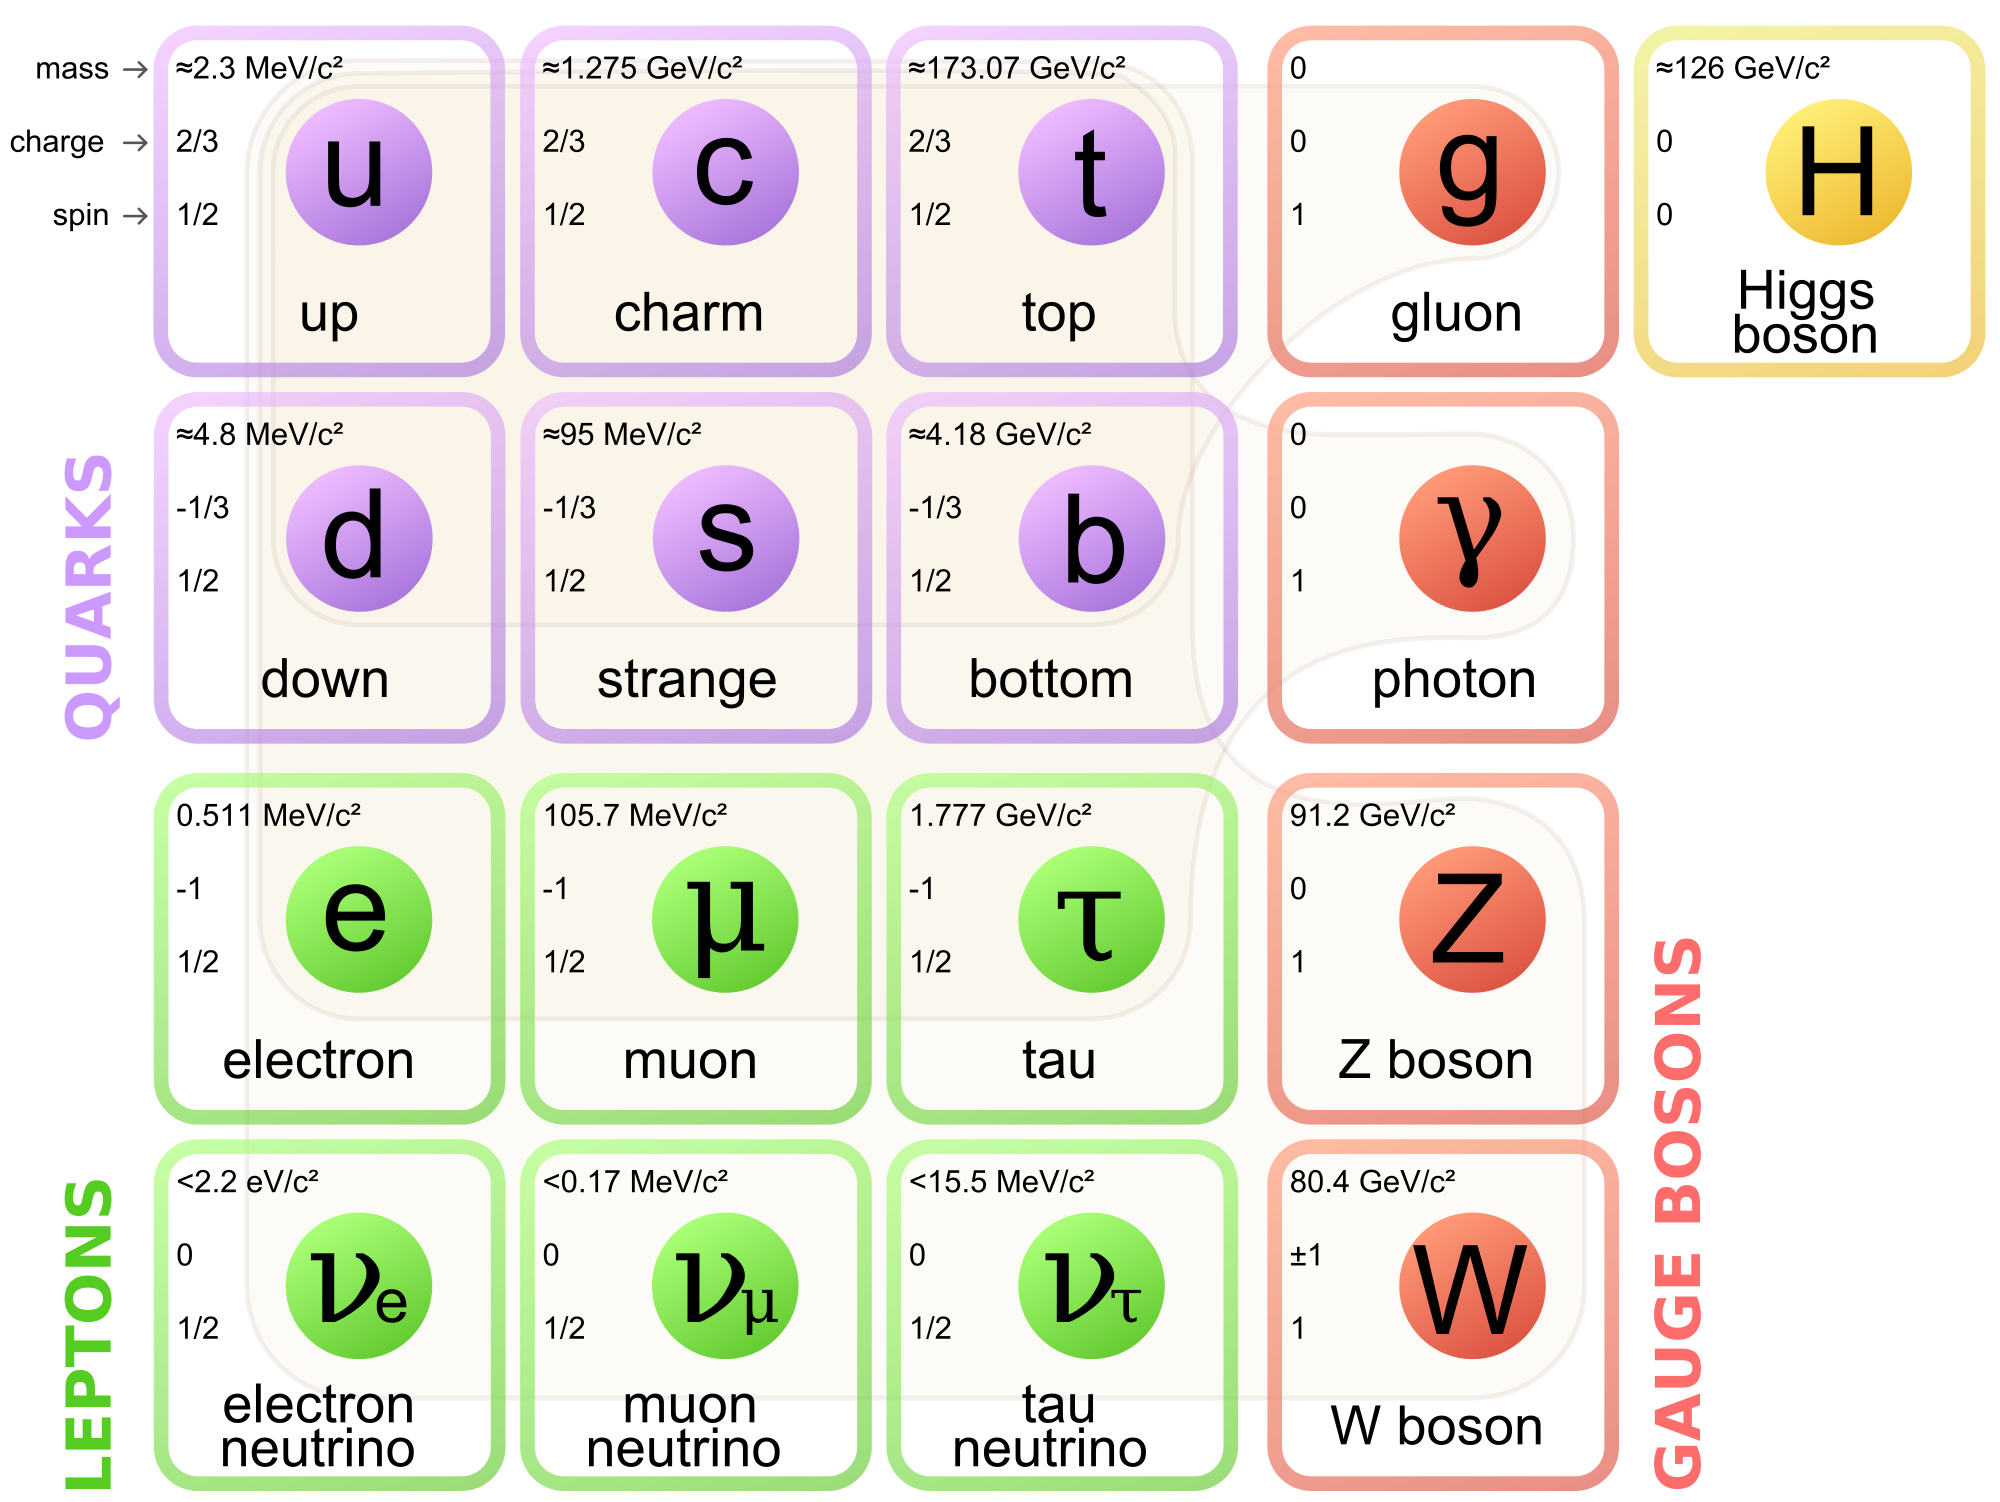
\includegraphics[width=0.6\textwidth]{01_Theory_SM/plots/Standard_Model_of_Elementary_Particles.png}
  \caption{The Standard Model of Elementary Particle Physics with three generations of matter fermions, gauge bosons and a Higgs boson. 
  The properties of the particles are also shown in each box.}
  \label{fig:SM_Particles}
\end{figure}


\subsection{Leptons}

The two bottom rows of fermions in the Fig.\ref{fig:SM_Particles} represent the known \textit{leptons} with their masses, charges
and spins. 

In general, the fermions are described with the Dirac equation\cite{diraceq}, which has 
% \begin{equation}\label{eq:dirac}
%   i\hbar\gamma^{\mu}\partial_{\mu}\psi - mc\psi = 0 ,
% \end{equation}
% 
% where the $\psi$ is a four-element Dirac spinor, an equivalent of a one dimentional Schr\"{o}dinger wave function, 
% $\gamma^{\mu}$s are the gamma matricies and $\partial_{\mu}$ is a partial derivative with respect to the time-space four-vector
% components. 
% 
solutions with positive and also with negative energy states. The latter are treated
as \textit{antiparticles}. So every lepton, being a fermion, has an antiparticle. In Fig.\ref{fig:SM_Particles}
only particles are shown. The electron $e^{-}$ has an antiparticle, called positron $e^{+}$. The muon $\mu^{-}$, tau $\tau^{-}$ and
their antiparticles, $\mu^{+}$ and $\tau^{+}$ differ from the electron and positron by their masses and their lifetimes.

Neutral leptons, neutrinos $\nu$, also have antiparticles, antineutrinos $\bar{\nu}$. Every massive lepton has a corresponding
neutrino: $\nu_{e}$, $\nu_{\mu}$ and $\nu_{\tau}$. Each type of the leptons has a lepton number (an electron and an electron neutrino 
have a lepton number $l_{e}$, muon and it's neutrino have a lepton number $l_{\mu}$ and the $\tau$ with it's neutrino have the 
lepton number $l_{\tau}$).  In this rule leptons have positive lepton numbers and
antileptons -- negative ones. The lepton number is conserved during the interactions.

\subsection{Quarks}\label{sec:quark}

The two upper rows in the Fig.\ref{fig:SM_Particles} list the known \textit{quarks}, showing their masses, charges and spins.

Quarks, being fermions, are also described by the Dirac equation. However, there is a number of properties which are very different
to the leptons. They have non-integer electric charge ($\frac{2}{3} e$ or $-\frac{1}{3} e$, where $e$ is the electron charge) and a 
\textit{flavour} (up, down, charm, strange, top and bottom).

Quarks have another charge called \textit{color}. All the observed isolated objects can't have color, they are colorless. Thus, the 
quarks have never been observed in an isolated state. The systems of bound quarks are called \textit{hadrons}. The most elementary hadrons are 
\textit{baryons}, which consist of three quarks, and \textit{mesons}, which consist of a quark and antiquark. The only stable yet known baryon 
is the proton. All the mesons are unstable.

The baryons are fermions as they consist of an odd number of quarks which have spins $\frac{1}{2}$. Thus, the mesons have integer spins
(0 or 1). This means that mesons are bosons.

\section{Interactions}

An interaction is the way the particles effect upon another particles and objects in their environment. The interaction is performed through exchange
of mediator bosons.

Nowadays only four basic interactions are known: \textit{strong}, \textit{electromagnetic}, \textit{weak} and \textit{gravity}. 
Each of them can be characterized by a \textit{strength}\footnote{A $strength$\cite{griffiths2008introduction} of the four basic forces can be determined as the value of each force
between two objects with given masses and charges and placed on a distance $r$ between each other. After all, the strength is an ambiguous notion, as the 
value of the force depends on the nature of the interacting objects and on the distance between them -- we can get different orders of strength on different
distances  and between different objects. The strength should not be understood literally, but just as a measure of order.}.
The following table shows the rough order of the interaction strengths, the mediator
and the theory, which describes these interactions \cite{griffiths2008introduction}:

\begin{center}\label{tab:forces}
  \begin{tabular}{ | c | c | c | c | }
    \hline
    \textbf{Interaction} & \textbf{Strength} & \textbf{Theory} & \textbf{Mediator} \\ \hline \hline
    Strong & 10 & Quantum Chromodynamics & Gluon \\ \hline 
    Electromagnetic & 10$^{-2}$ & Quantum Electrodynamics & Photon \\ \hline
    Weak & 10$^{-13}$ & Flavordynamics & $W$ and $Z$ Bosons \\ \hline
    Gravitation & 10$^{-42}$ & Geometrodynamics & Graviton \\
    \hline
  \end{tabular}
\end{center}

All the equations and values listed in this work are presented assuming that $\hbar = c = 1$. This is called the \textit{natural units}. 
More details on every interaction is presented in the following section.

\subsection{Electrmagnetic Interaction}

The theory behind the electromagnetic interactions -- quantum electrodynamics (QED) -- was developed earlier than other interactions theories
and is the most successful one. It describes the interactions between the elementary electrically charged fermions via mediator photons.
The electromagnetic interaction is such that the oppositely electrically charged objects attract each other while same sign charges repulse.
This interaction is present at any distance, getting weaker proportionally to the distance squared. QED is based on the gauge group $U(1)$.
Every electromagnetic phenomena is ultimately reducible to the following elementary process:

\begin{figure}[h]
  \centering
  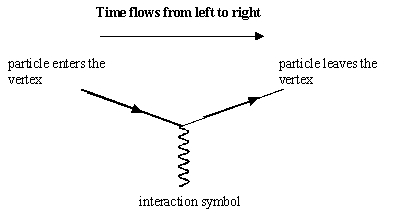
\includegraphics[width=0.6\textwidth]{01_Theory_SM/plots/QED_simple.png}
  \caption{Feynman graph of the elementary QED process.}
  \label{fig:QED_simple}
\end{figure}

The more complex processes can be described combining two or more of these elementary vertices.

The coupling constant, or the interaction strength of the electromagnetic interaction is given as following:

\begin{equation}
 \alpha = \frac{e^{2}}{4\pi\epsilon_{0}} \approx \frac{1}{137},
\end{equation}

where $\epsilon_{0}$ is the permitivity of vacuum, $e$ is the electron charge and $c$ is the speed of light.

As the coupling constant is small ($\alpha \ll 1$), it can be used for expansion in perturbative calculations (observable ~ $\sum_{k=0}^{\infty} c_{k}\cdot\alpha^{k}$).
The naming of the processes lying beyond each of the terms of the expansion
is Leading Order process (LO, which takes into account the first term with non-zero $c_{k}$), Next-to-Leading Order process (NLO, also takes
to account the next term, additionally to the LO), Next-to-Next-to-Leading Order process (NNLO), etc.

\subsection{Strong Interaction}\label{sec:strong_int}

The theory which describes the strong interaction is Quantum Chromodynamics (QCD), which is based on the gauge group $SU(3)$. Only the
objects which have a color charge can interact strongly. The color charge (first mentioned in sec. \ref{sec:quark}) has three eigenstates:
red (r), blue (b) and green (g). As for the any other charge, the color charge eigenstates have also anticharges -- anticolors. The combination
of the color and corresponding anticolor, as well as the combination of all the colors/anticolors results in colorless states.

The mediators of the strong interaction are gluons. These particles are massless and carry two colors -- color and anticolor. Thus, the strong 
interaction is the interaction between quarks via gluons. The color charge is conserved during the interaction.

The coupling constant of the strong interaction, $\alpha_{s}$, is a running constant depending on the energy scale $Q$. As shown in the
Fig. \ref{fig:Alpha_s}, $\alpha_{s}$ rapidly increases with the lessening of $Q$. This means that at larger distances 
the strength of the interaction increases a lot. This phenomenon is called \textit{confinement} and this is the reason why the quarks
can't exist in an isolated state. The more the quarks separate from each other in terms of distance, the stronger they interact, the harder
it becomes to separate them further. Even if one always has enough energy to separate quarks more and more from each other, they gluon field will become critically
high and produce a quark-antiquark pair. This process may repeat sequentially. This constantly happens under the conditions created in the
particle colliders. The phenomenon of sequential quark pair production is called \textit{hadronization}.

The confinement constrains the maximum distances on which the interaction in terms of the gluon field is observed before producing a quark-antiquark pair.
The limit of the region of strong interaction impact is of the order of the nucleon size $\sim 10^{-15}$ m.

\begin{figure}[t]
  \centering
  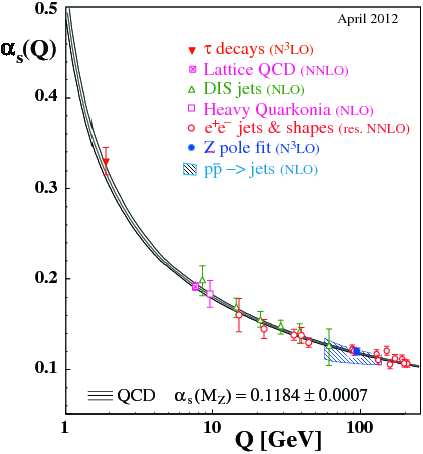
\includegraphics[width=0.6\textwidth]{01_Theory_SM/plots/Alpha_s.png}
  \caption{Summary of measurements of $\alpha_s$ as a function of the respective energy scale $Q$. The respective degree of QCD perturbation 
  theory used in the extraction of $\alpha_{s}$ is indicated in brackets (NLO: next-to-leading order; NNLO: next-to-next-to leading order; 
  res. NNLO: NNLO matched with resummed next-to-leading logs; N3LO: next-to-NNLO). Figure taken from \cite{PDG-2012}.}
  \label{fig:Alpha_s}
\end{figure}

The opposite tendency which can be observed in Fig. \ref{fig:Alpha_s} is that the $\alpha_{s}$ is getting smaller for higher values 
of the $Q$. This means that for the shorter interaction distances, the coupling constant becomes weaker. This phenomenon carries the 
name \textit{asymptotic freedom}\cite{PhysRevLett.30.1343}. Under these conditions the quarks are assumed to be treated as the free particles. The asymptotically 
free quarks are assumed to be observed in the \textit{quark-gluon plasma} \cite{Bohr1977275} -- the state of matter with extremely high density and/or temperature.

% The conjectured QCD states, depending on temperature and density, are shown in Fig. \ref{fig:QGP}.

% \begin{figure}[t]
%   \centering
%   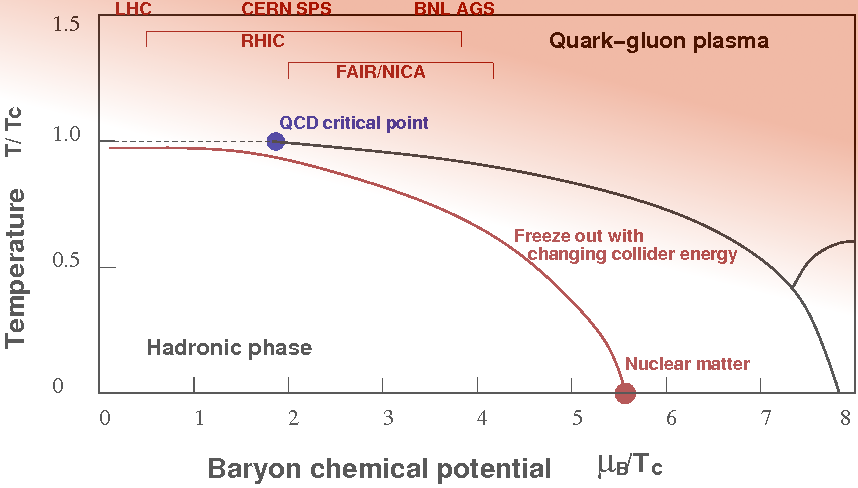
\includegraphics[width=0.8\textwidth]{01_Theory_SM/plots/QGP.png}
%   \caption{Conjectured phase diagram of QCD. The different states and phase curves are shown. The energy and density range of different high energy 
%   physics experiments are marked on the top of the figure.}
%   \label{fig:QGP}
% \end{figure}

\subsection{Weak Interaction}

As it can be seen in the table \ref{tab:forces}, the strength of the weak interaction is many orders of magnitude smaller than the one for the 
electromagnetic and strong interaction. This fact explains the name \textit{weak}.

The weak interaction differs from the others in a way that there is no particular name for the charge responsible for this interaction 
(like electrical charge for the electromagnetism and color charge for the strong interaction). All the leptons and quarks carry the ability to interact
weakly. A widely known example of the weak interaction is the process of the $\beta$-decay. The lepton number and lepton flavour both conserve in the weak interaction.

There are two kinds of weak interaction: \textit{neutral}, mediated by the 
$Z$-bosons, and \textit{charged}, mediated by the $W^{\pm}$. The masses of the 
mediators are shown in the Fig. \ref{fig:SM_Particles}.	In the neutral weak interaction there is no charge as well as no quark flavour exchange between the 
interacting particles. In the charged weak interaction, both the charge and the quark flavour exchange, are present. In the charged weak interactions 
the quark flavour can exchange not only within one generation, but also between the generations.
This intergeneration flavour exchange wouldn't be allowed within the normal quark mass eigenstates:

\begin{equation}
\left( \begin{array}{c}
       u \\ d
      \end{array} \right)
\left( \begin{array}{c}
       c \\ s
      \end{array} \right)
\left( \begin{array}{c}
       t \\ b
      \end{array} \right)
\end{equation}
  
The weak quark eigenstates differ from the mass ones. For the former ones, the $d$, $s$ and $t$ states are replaced with their linear combinations $d'$, $s'$ and $b'$,
expressed as follows:

\begin{equation} \label{eq:CKM_transform}
\left( \begin{array}{c} d' \\ s' \\ b' \end{array} \right) = 
\left( \begin{array}{ccc} V_{ud} & V_{us} & V_{ub} \\ V_{cd} & V_{cs} & V_{cb} \\ V_{td} & V_{ts} & V_{tb} \end{array} \right)
\left( \begin{array}{c} d \\ s \\ b\end{array} \right).
\end{equation}

The matrix $V$ in \ref{eq:CKM_transform} is the Cabibbo-Kobayashi-Maskawa matrix \cite{Kobayashi:1973fv} (CKM-matrix), which describes the transition probability 
between different quark flavours. Experimentally defined, the matrix elements have the following magnitudes \cite{PDG-2012}:

\begin{equation} \label{eq:CKM}
 V = \left( \begin{array}{ccc} 0.974 & 0.225 & 0.003 \\ 0.225 & 0.973 & 0.041 \\ 0.009 & 0.040 & 0.999 \end{array} \right).
\end{equation}

The diagonal elements of the CKM matrix (\ref{eq:CKM}) are close to 1, being much higher than the off-diagonal elements. Thus, flavour transformations
within one generation are preferred.

As the masses of the gauge bosons which mediate the weak interaction are quite large (see Fig. \ref{fig:SM_Particles}), the range of the interaction is restricted
to a size of $\sim \frac{\hbar}{M_{W}c}$.

\subsection{Electroweak Unification and Symmetry Breaking}

If one compares the neutral weak interactions and the electromagnetic ones, it becomes obvious that they are very similar, differing mainly on the mediator
of the interaction. This can be also seen in Fig. \ref{fig:em_weak}.

\begin{figure}[h]
  \centering
  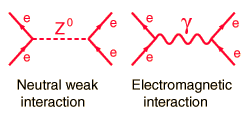
\includegraphics[width=0.6\textwidth]{01_Theory_SM/plots/feynz.png}
  \caption{$ee$ scattering in the electromagnetic (right) and neutral weak (left) interactions.}
  \label{fig:em_weak}
\end{figure}

A unification of these two interactions would seem to be a natural idea. It is not that simple as replacing the $Z^{0}$ by the photon $\gamma$, one
should take to account both processes and their interferences.

The theory which describes the unified electroweak interactions is based on the $SU(2) \times U(1)$ symmetry. To make the Lagrangian of the weak interaction
symmetric to the $SU(2)$ transformations, three fields are introduced: $W_{\mu}^{1}$, $W_{\mu}^{2}$ and $W_{\mu}^{3}$. These fields couple to fermions with
the coupling constant $g$. The fields $W_{\mu}^{1}$ and $W_{\mu}^{2}$ couple to the left-handed\footnote{The \textit{chirality} of the particle defines it's handnessness.
The left-handed and right-handed states are the different components of the Dirac spinor\cite{aitchison2003gauge}. The parity transformation change the chirality (from
left-handed to right handed and vise versa). For the massless particles chirality is the same as helicity -- the property of the particle, which describes the coincide
of the spin and motion directions.} fermions and
the $W_{\mu}^{3}$ is coupling to the neutrinos. The $W^{\pm}$ couples to the left-handed fermions, thus it can be represented as a linear combination of
$W_{\mu}^{1}$ and $W_{\mu}^{2}$:

\begin{equation}
 W^{\pm} = \frac{1}{\sqrt{2}}(W_{\mu}^{1} \mp iW_{\mu}^{2}).
\end{equation}

The symmetry $U(1)$ introduces the additional field $B_{\mu}$ which couples to neutrinos. The related coupling constant is $g'$. To describe the electromagnetic
field, the $Z_{\mu}$ and $\gamma_{\mu}$ fields are introduced:

\begin{equation}\label{eq:Zmu}
 Z_{\mu} = \frac{1}{\sqrt{g^{2} + g'^{2}}}(gW^{3}_{\mu} - g'B_{\mu}),
\end{equation}

\begin{equation}\label{eq:Amu}
 \gamma_{\mu} = \frac{1}{\sqrt{g^{2} + g'^{2}}}(gW^{3}_{\mu} + g'B_{\mu}).
\end{equation}

A free parameter of the Standard Model, which is introduced in this context, is the weak mixing angle $\theta_{W}$, which is expressed as follows:

\begin{equation}
 cos(\theta_{W}) = \frac{g}{\sqrt{g^{2}+g'^{2}}}.
\end{equation}

Thus, the fields $Z_{\mu}$ and $\gamma_{\mu}$ can be expressed via this angle:

\begin{equation}
 Z_{\mu} = W^{3}_{\mu}cos(\theta_{W}) - B_{\mu}sin(\theta_{W}),
\end{equation}

\begin{equation}
 \gamma_{\mu} = W^{3}_{\mu}cos(\theta_{W}) + B_{\mu}sin(\theta_{W}).
\end{equation}

So in fact, the photon $\gamma$ and the $Z^{0}$ mix the states of $W^{3}_{\mu}$ (corresponding to $W^{0}$) and $B_{\mu}$ (corresponding to $B^{0}$).
The mixing angle $\theta_{W}$ has been measured experimentally \cite{PDG-2012} and corresponds to approximately $30^{o}$.

There is also a charge introduced to describe the electroweak interaction, which is called a \textit{hypercharge} $Y$ and is expressed in the Gell-Mann--Nishijima
equation:

\begin{equation}
 Y = (2Q - I_{3}).
\end{equation}

Here $Q$ is an electric charge in units of the electron charge $e$ and $I_{3}$ is the weak isospin.

The whole model, however, is based on the assumption that all gauge bosons have to be massless, which is not the case. The known experimental fact
is that the $W^{\pm}$ and $Z^{0}$ bosons carry a non-zero mass \cite{PDG-2012}. The masses appear in this theory due to \textit{spontaneous gauge symmetry
breaking}. In another words, the particles remain massless, but a new field appears. The particles couple to this field and obtain masses in this
interaction. The symmetry breaking is accompanied with the appearance of one or two massless particles with zero spin, so-called \textit{Goldstone bosons}.
They are eliminated by the \textit{Higgs mechanism}\cite{1964PhRvL..13..508H}, which, however, introduces a massive particle with zero spin - \textit{Higgs boson}. At the time when the
Higgs mechanism was introduced, such particle was not yet discovered. A Higgs-like particle was discovered only in 2012 \cite{Aad20121, Chatrchyan:2012xdj} 
and it's properties still need to be checked for the consistency to the theoretical predictions.


\subsection{Gravity}

The fourth interaction which is present in our Universe is gravity. The gravity is not described in Standard Model, but it has to be mentioned for a consistent 
picture. The gravity is described by the \textit{general relativity}, which is a classical non-quantum field theory. Up to now it couldn't be matched with the
Standard Model. The Standard Model breaks down at the large scale, where gravity starts to play role. Although the extension of the Standard Model is predicting 
the existence of a gravity gauge boson - a \textit{graviton} with a spin 2 and zero mass. However, there has been no experimental proof of it's existence to date.

The gravitation force is very weak on the small distances, which are typical for the interaction of elementary particles. It only becomes noticable
on a very large distance. For example, the movement of the bodies in outer space (planets, stars, asteroids, etc) are to the large extend governed by
gravity.

The "charge`` which reacts to the gravity is the mass of the body. 

The influence of gravity is negligible for the processes studied in this thesis, thus it is neglected.

\section{Top Quark Physics}

In this thesis the process of $t\bar{t}$ production is being analyzed. Thus, some more details of the top quark physics should be presented.
The top quark has unique properties compared to the other elementary particles: it is the heaviest known elementary particles and it decays 
faster than it can hadronize. Thus, it offers possibilities for numerous studies. Studying the top quark is gaining knowledge about a bare quark, 
which is not possible to do with any other quark. This section describes the production process of the top quark and its decay.

\subsection{Top Quark Production}\label{ssec:tprod}

The top quark production cross section depends on the center-of-mass energy of the experiment in which it is produced. From Fig. \ref{fig:SM_XSec_Prod}
one can judge that under the conditions of the Large Hadron Collider (where the designed center-of-mass energy should approach 14 TeV) acts like 
a top production factory. The top production cross section ($\sigma_{top}$) at the LHC scale is almost an order of magnitude larger than for the
TEVATRON.

\begin{figure}[p]
  \centering
  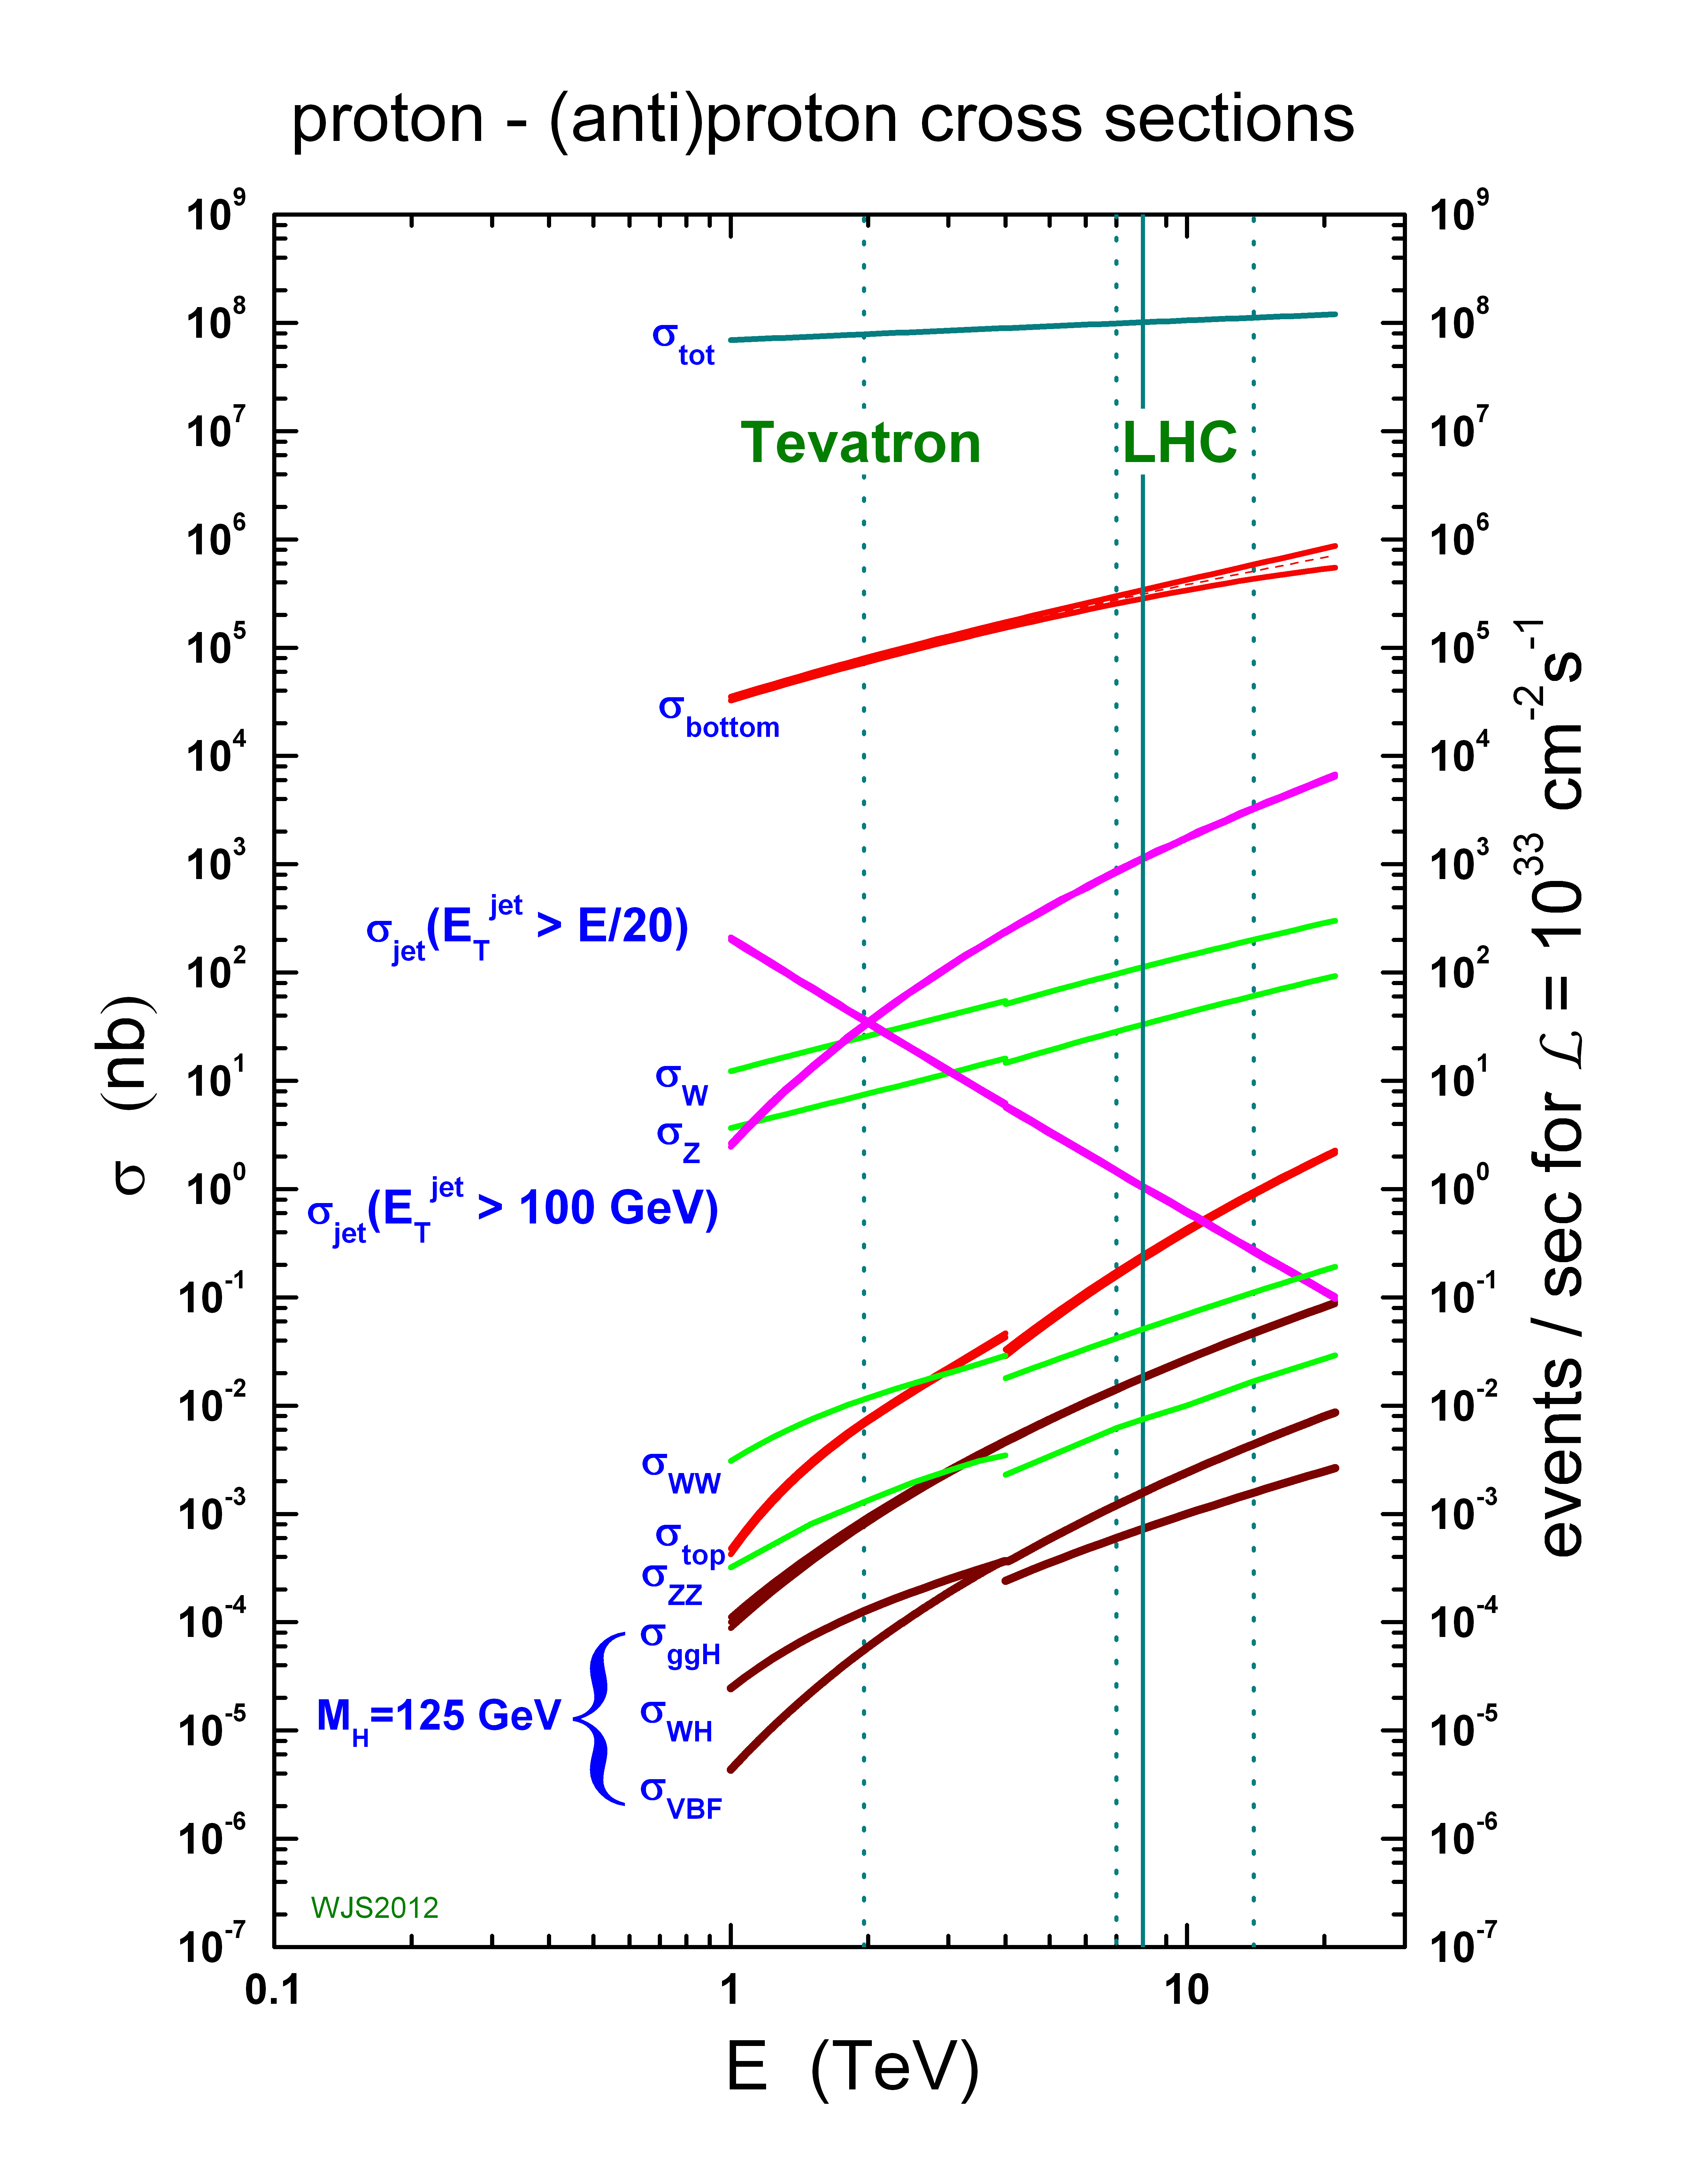
\includegraphics[width=1.0\textwidth]{01_Theory_SM/plots/crosssections2013.png}
  \caption{Standard Model Leading Order cross sections for the different processes depending on the energies. The turquoise vertical line presents the energy
  of the Large Hadron Collider running in 2012.}
  \label{fig:SM_XSec_Prod}
\end{figure}

The top quarks may be produced as single top quarks or in pairs.

\subsubsection{Top Quark Pair Production}

The dominant $t\bar{t}$ production mechanism in SM is the one via strong interaction. In the QCD the inclusive production cross section of the $t\bar{t}$ pair
from the proton-proton interaction can be expressed as follows \cite{Schilling:2012dx}:

\begin{equation} \label{eq:pptt}
 \sigma_{pp \rightarrow t\bar{t}} (s, m_{t}) = \sum_{i,j = q, \bar{q}, g} \int dx_{i} dx_{j} f_{i}(x_{i}, \mu_{f}^{2}) f_{j}(x_{j}, \mu_{f}^{2}) \cdot \hat{\sigma}_{ij \rightarrow t\bar{t}}(\hat{s}, m_{t}, \mu_{f}, \mu_{r}, \alpha_{s}).
\end{equation}

Here the sum is running over all quarks and gluons contributing to the process, $m_{t}$ is the mass of the top quark, $s$ is the squared center-of-mass 
energy for the $pp$ collision, $x$ is the parton momentum fractions with respect to the proton momenta, $\mu_{f,r}$ are the factorization and renormalization 
scales, $\hat{s} \sim sx_{i}x_{j}$ is the partonic center-of-mass energy, $\alpha_{s}$ is the strong coupling constant and  $f(x, \mu_{f}^{2})$ is the parton distribution
function (PDF). 

The formula \ref{eq:pptt} is a convolution of the proton densities and hard scattering cross sections. As the mass of the $t\bar{t}$ pair is high, the $\alpha_{s}$ turns out
to be quite low (see Fig. \ref{fig:Alpha_s}), thus the perturbative expansion of the hard scattering cross sections is possible.
The \textit{Parton Distribution Function}, or the \textit{PDF}, is depending on the parton flavour $i$, parton momentum
fraction $x_{i}$ and the energy scale of the interaction. A PDF gives a probability that within the interaction of a given scale a parton with a given flavour $i$
and momentum fraction $x_{i}$ will be found in a proton. According to the DGLAP evolution\cite{Altarelli:1977zs, Dokshitzer:1977sg, Gribov:1972ri}, it is a sum of the 
densities of all the quark (valent and from the sea) and gluon constituents. 

The proton densities can not be calculated in the perturabtive QCD. They are obtained as a result of experimental data fit.
The PDFs are measured by different groups (for example, HERAfitter \cite{Alekhin:2014irh} or 
CTEQ \cite{Pumplin:2002vw}). An example of the combined HERA PDFs is shown in Fig. \ref{fig:HERA_PDF}.

\begin{figure}[t]
  \centering
  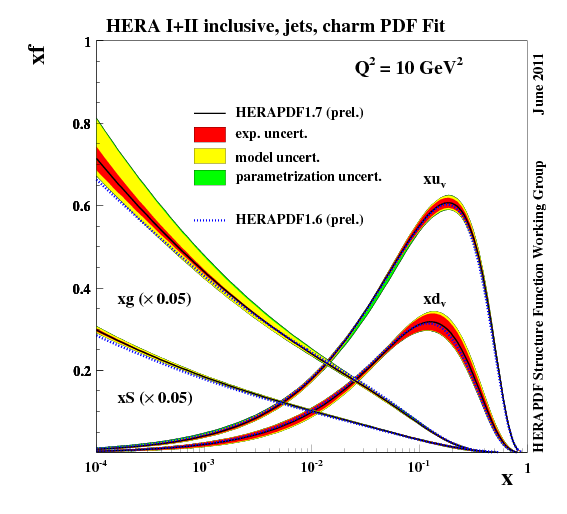
\includegraphics[width=0.8\textwidth]{01_Theory_SM/plots/herapdf17.png}
  \caption{PDFs from HERAPDF1.7, which includes charm data, jet data and low energy data as well as the HERA-I and II high energy inclusive data.}
  \label{fig:HERA_PDF}
\end{figure}

The $t\bar{t}$ pairs are dominantly produced in the process of gluon-gluon fusion $gg \rightarrow t\bar{t}$ or in quark-antiquark annihilation $q\bar{q} \rightarrow t\bar{t}$.
These LO production processes are shown in Fig. \ref{fig:LO_tt_prod}. In the NLO production processes there are also partonic sub-processes with $gq$($g\bar{q}$) present.

\begin{figure}[h]
  \centering
  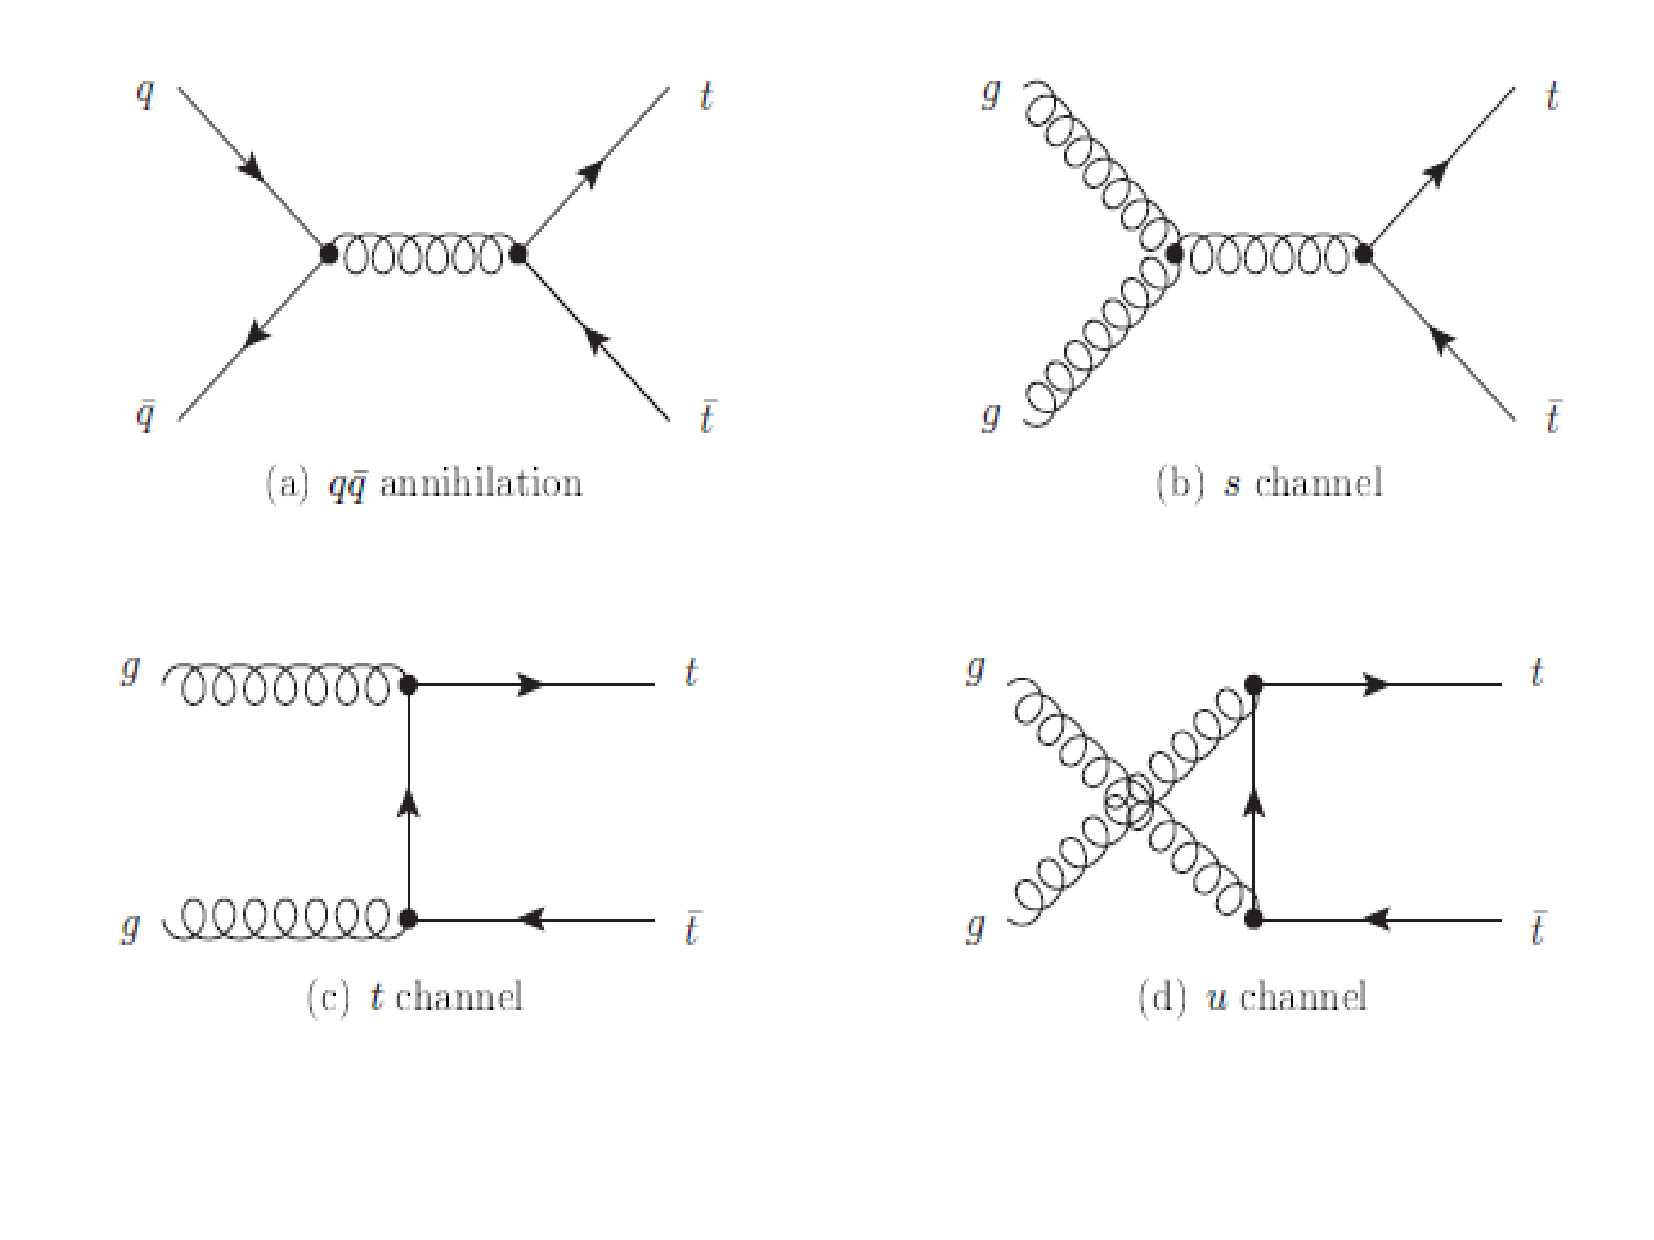
\includegraphics[width=0.8\textwidth]{01_Theory_SM/plots/LO_tt_production.pdf}
  \caption{Feynman diagrams for the LO $t\bar{t}$ production.}
  \label{fig:LO_tt_prod}
\end{figure}

\subsubsection{Single Top Production}

The top quarks can be also produced not in pairs in the weak interaction processes in the $Wtb$ vertex.

There are three production modes of the single top -- $t$-channel, $s$-channel and $tW$-channel. These production channels are shown in Fig. \ref{fig:single_t_prod}.

\begin{figure}[h]
  \centering
  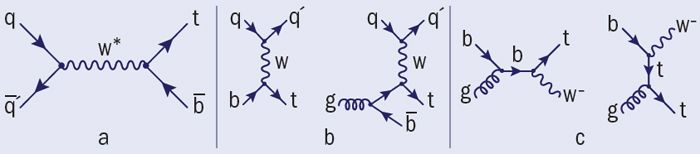
\includegraphics[width=0.8\textwidth]{01_Theory_SM/plots/single_top.png}
  \caption{Feynman diagrams for the LO single $t$-quark production. Three different production channels for single top quarks are illustrated: 
  the $s$-channel (a), the $t$-channel (b) and the W-associated $tW$-channel (c).}
  \label{fig:single_t_prod}
\end{figure}

Single top quark production is interesting for various studies. It is a test of Standard Model and it is directly sensitive to the CKM matrix
element $|V_{tb}|$.

\subsection{Top Quark Pair Decay}\label{ssec:tdecay}

The top quark decays before hadronizing almost exclusively to a $b$-quark and a $W$-boson, as the value of $|V_{tb}|$ is almost 1 (see CKM matrix \ref{eq:CKM}).

The decay modes of the $t\bar{t}$ pairs can be classified according to the decay mode of the $W$ bosons (see Fig. \ref{fig:tt_decay}):

\begin{figure}[h]
\centering
\begin{subfigure}
  \centering
  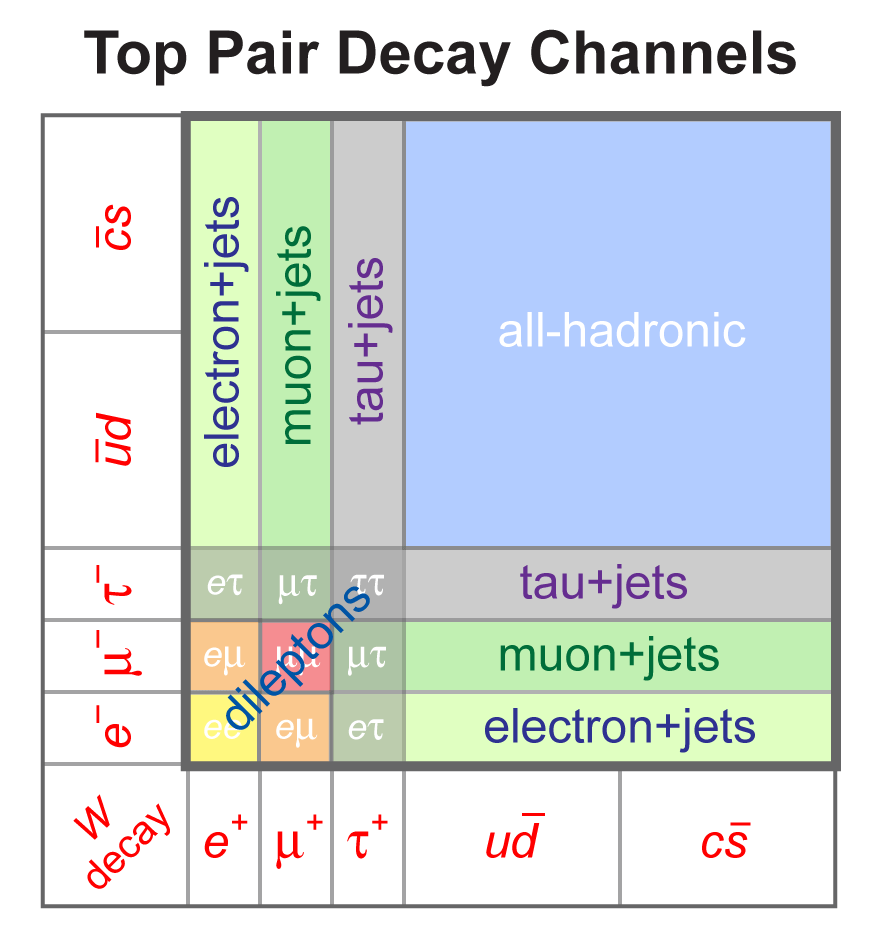
\includegraphics[width=0.49\textwidth]{01_Theory_SM/plots/top_pair_decay_channels.png}
\end{subfigure}
\begin{subfigure}
  \centering
  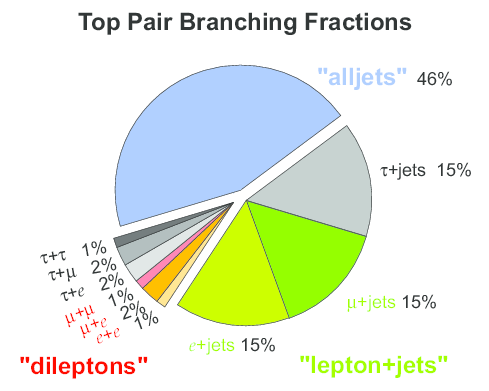
\includegraphics[width=0.49\textwidth]{01_Theory_SM/plots/top_pair_branching_frac.png}
\end{subfigure}
\caption{$t\bar{t}$ decay channels. On the right the branching ratio of different decay channels are shown.}
  \label{fig:tt_decay}
\end{figure}

\begin{itemize}
 \item \textit{Full hadronic channel}. Both $W$ bosons decay into quark-antiquark pairs -- $t\bar{t} \rightarrow (W^{+} \rightarrow q\bar{q}')b\:(W^{-} \rightarrow q''\bar{q}''')\bar{b}$.
 This decay channel has the largest branching ratio\footnote{\textit{Branching ratio} of the specific decay of a particular particle/system is the probability of this particle/system
 to decay via this decay mode.}. However, this state has a very high pollution in the Large Hadron Collider environment, as the large number of quark and gluon jets is produced.
 
 \item \textit{Semileptonic (lepton+jet) channel}. One $W$ boson decays hadronically, another one - into two leptons:  $t\bar{t} \rightarrow (W^{\pm} \rightarrow q\bar{q}')b \: (W^{\mp} \rightarrow l^{\mp}\nu)\bar{b}$.
 The high momentum lepton, which occurs in this process, is a signature that helps to identify the decay better. Thus, there is less
 ambiguity in defining the final state of the semileptonic $t\bar{t}$ decay.
 
 \item \textit{Dileptonic channel}. Both $W$ bosons decay into leptons -- $t\bar{t} \rightarrow (W^{+} \rightarrow l^{+}\nu_{l^{-}})b \: (W^{-} \rightarrow l^{-}\bar{\nu}_{l^{-}})\bar{b}$.
 This decay channel has the smallest branching ratio, but the two high momentum leptons are a nice sign which helps to distinguish this final state from other processes
 occurring in the Large Hadron Collider collisions.
\end{itemize}

This analysis is based on the dileptonic channel. However, only the final states where the electrons or/and muons occur are considered. The once with $\tau$ leptons are 
not taken to account as signal.

\subsection{Studies of the $t\bar{t}$ Production}

The studies of the $t\bar{t}$ production process provide a very important test of the Standard Model. 

In particular, the $t\bar{t}$ production in the $pp$ collisions at the LHC is dominated by gluon-gluon fusion (sec. \ref{ssec:tprod}, fig.\ref{fig:LO_tt_prod}), which 
is precisely measured in the QCD. Thus, the $t\bar{t}$ production cross section measurement can provide constrains for the PDF and the strong coupling constant $\alpha_s$.
The total $t\bar{t}$ production cross section is accurately calculated up to NNLO, which means that the experimental measurement of this cross sections provide a 
test of perturbative QCD.
On the other hand, the deviation from the QCD predictions may point to some processes beyond the Standard Model, as, e.g., to the SUSY particles production, which decay
to the $t\bar{t}$ pairs. In addition, a measurement of the $t\bar{t}$ production cross sections may deliver information about various top properties, e.g. mass or spin
of the $t$-quark.